\documentclass[12pt,a4paper]{scrartcl}
\usepackage[utf8]{inputenc}
\usepackage[ngerman]{babel}
\usepackage{amsmath}
\usepackage{amsfonts}
\usepackage{amssymb}
\usepackage{color}
\usepackage{graphicx}
%\usepackage{listings}
\usepackage[left=2.5cm, right=2cm, top=2cm, bottom=2cm]{geometry}

\usepackage[hidelinks]{hyperref}
\usepackage{scrpage2}
\usepackage{csquotes}
\usepackage{subcaption}


\DeclareUnicodeCharacter{00A0}{ }

\pagestyle{scrheadings}


\linespread{1.5}
\setlength{\parindent}{0cm} % No paragraph indent


\newcommand{\q}[1]{``#1''}
\newcommand{\todo}[1]{\begin{Large}\textcolor{red}{$\Rightarrow ~$#1}\end{Large}}

\newcommand{\ant}[1]{\begin{Large}\textcolor{green}{$\Rightarrow ~$#1}\end{Large}}


\newcommand{\inmilestonetwo}{\vspace{0.75cm} \framebox[1.1\width]{
\begin{large}
\textcolor{red}{Die Dokumentation dieses Abschnittes ist für Milestone II vorgesehen.}
\end{large}}}



\begin{document}

% University Assignment Title Page 
% LaTeX Template
% Version 1.0 (27/12/12)
%
% This template has been downloaded from:
% http://www.LaTeXTemplates.com
%
% Original author:
% WikiBooks (http://en.wikibooks.org/wiki/LaTeX/Title_Creation)
%
% License:
% CC BY-NC-SA 3.0 (http://creativecommons.org/licenses/by-nc-sa/3.0/)
% 

\begin{titlepage}

\newcommand{\HRule}{\rule{\linewidth}{0.5mm}} % Defines a new command for the horizontal lines, change thickness here

\center % Center everything on the page
 
%----------------------------------------------------------------------------------------
%	HEADING SECTIONS
%----------------------------------------------------------------------------------------

\textsc{\LARGE Programmierprojekt}\\[1.5cm] % Name of your university/college
\textsc{\Large Alte Kantonsschule Aarau}\\[0.5cm] % Major heading such as course name
\textsc{\large}\\[0.5cm] % Minor heading such as course title

%----------------------------------------------------------------------------------------
%	TITLE SECTION
%----------------------------------------------------------------------------------------

\HRule \\[0.4cm]
{ \huge \bfseries Dokumentation: Spacetraveler}\\[0.4cm] % Title of your document
\HRule \\[1.5cm]
 
%----------------------------------------------------------------------------------------
%	AUTHOR SECTION
%----------------------------------------------------------------------------------------

\begin{minipage}{0.4\textwidth}
\begin{flushleft} \large
\emph{Autoren:}\\
Gabriel \textsc{Gavrilas}\\ % Your name\\
Patrick \textsc{Eigensatz}\\ % Your name\\
Jonas \textsc{Wahlen}\\ % Your name\\
\end{flushleft}
\end{minipage}
~
\begin{minipage}{0.4\textwidth}
\begin{flushright} \large
%\emph{Betreuer:} \\
%Dr. Martin \textsc{Jordi} % Supervisor's Name
\end{flushright}
\end{minipage}\\[2cm]

% If you don't want a supervisor, uncomment the two lines below and remove the section above
%\Large \emph{Author:}\\
%John \textsc{Smith}\\[3cm] % Your name

%----------------------------------------------------------------------------------------
%	DATE SECTION
%----------------------------------------------------------------------------------------

{\large Februar 2016}\\[2cm] % Date, change the \today to a set date if you want to be precise

%----------------------------------------------------------------------------------------
%	LOGO SECTION
%----------------------------------------------------------------------------------------

%\includegraphics[width=12cm]{img/titelbild.jpg}\\[1cm] % Include a department/university logo - this will require the graphicx package
 
%----------------------------------------------------------------------------------------

\vfill % Fill the rest of the page with whitespace

\end{titlepage}

\clearpage

\tableofcontents

\clearpage

\todo{Informationen / Beispielarbeit beachten!}

\section{Projektbeschreibung}
\subsection{Spielidee}
Ziel unseres Spieles ist es, dass der Spieler sein Raumschiff von einer Startposition im Level
zum Ziel bringt. Dazu eine kleine Story:
\todo{Story erstellen}
\begin{verbatim}
Der Wissenschaftler Dr. xy ist mit seiner Gravitationskanone...
\end{verbatim}

\subsection{Physik}
\subsection{Gravitation}

\subsection{Kollision}




\section{Problemdefinition}
\subsection{Grundkriterien}
Wir haben uns folgende Grundkriterien gesetzt:
\begin{itemize}
\item Gravitation: Punkte, die den Spieler unterschiedlich stark gegen sich ziehen.
\item Der Spieler ist ein Raumschiff.
\item Der Spieler befindet sich in einem Raum fernab von jeder anderen Kraftquelle ausserhalb des Levels.
\item Der Spieler bewegt sich durch dieses Level mithilfe von  einem Gravitationspunkt, den er platzieren und entfernen kann; Er kann sich also \q{in eine Richtung ziehen lassen}
\item Das Level ist beschränkt, hat also einen Start und ein Ziel
\item Es gibt Wände, die den Raum beschränken.
\end{itemize}

\subsection{Zusatzkriterien}
Als Zusatzkriterien setzen wir uns weiter:
\begin{itemize}
\item Gegner und/oder Hindernisse (= Objekte bei deren Kollision der Spieler stirbt) z.B: Asteroiden die sich frei bewegen, oder sehr starke Gravitationszentren, die den Spieler gegen ein Objekt ziehen und so eine Kollision auslösen.
\item Gameover-Grafik, die angezeigt wird, wenn der Spieler stirbt oder die Zeit abläuft.
\item Es besteht eine kleine Reibung, die den Spieler leicht abbremst.
\item Zeitliche Beschränkung (z.B: 2min, wenn Zeit = 0, ist das Spiel zu Ende)
\item Startmenu und Spielanleitung
\end{itemize}

\subsection{Grundkriterien}
Wir haben uns folgende Grundkriterien gesetzt:
\begin{itemize}
\item Gravitation: Punkte, die den Spieler unterschiedlich stark gegen sich ziehen.
\item Der Spieler ist ein Raumschiff.
\item Der Spieler befindet sich in einem Raum fernab von jeder anderen Kraftquelle ausserhalb des Levels.
\item Der Spieler bewegt sich durch dieses Level mithilfe von  einem Gravitationspunkt, den er platzieren und entfernen kann; Er kann sich also \q{in eine Richtung ziehen lassen}
\item Das Level ist beschränkt, hat also einen Start und ein Ziel
\item Es gibt Wände, die den Raum beschränken.
\end{itemize}

\subsection{Zusatzkriterien}
Als Zusatzkriterien setzen wir uns weiter:
\begin{itemize}
\item Gegner und/oder Hindernisse (= Objekte bei deren Kollision der Spieler stirbt) z.B: Asteroiden die sich frei bewegen, oder sehr starke Gravitationszentren, die den Spieler gegen ein Objekt ziehen und so eine Kollision auslösen.
\item Gameover-Grafik, die angezeigt wird, wenn der Spieler stirbt oder die Zeit abläuft.
\item Es besteht eine kleine Reibung, die den Spieler leicht abbremst.
\item Zeitliche Beschränkung (z.B: 2min, wenn Zeit = 0, ist das Spiel zu Ende)
\item Startmenu und Spielanleitung
\end{itemize}



\section{Anforderungsanalyse}
% maximal 2 sätze, in java realisierbar
Das Programm lässt sich mitsamt seinen Anforderungen vollständig in Java implementieren.
Es werden auf Soft-/Hardwareebene keine weiteren Anforderungen gestellt, als ein einfacher Computer mit
Maus und funktionierender JRE.


\section{Spezifikation}
\subsection{Use Cases}
\subsubsection{Spieler}
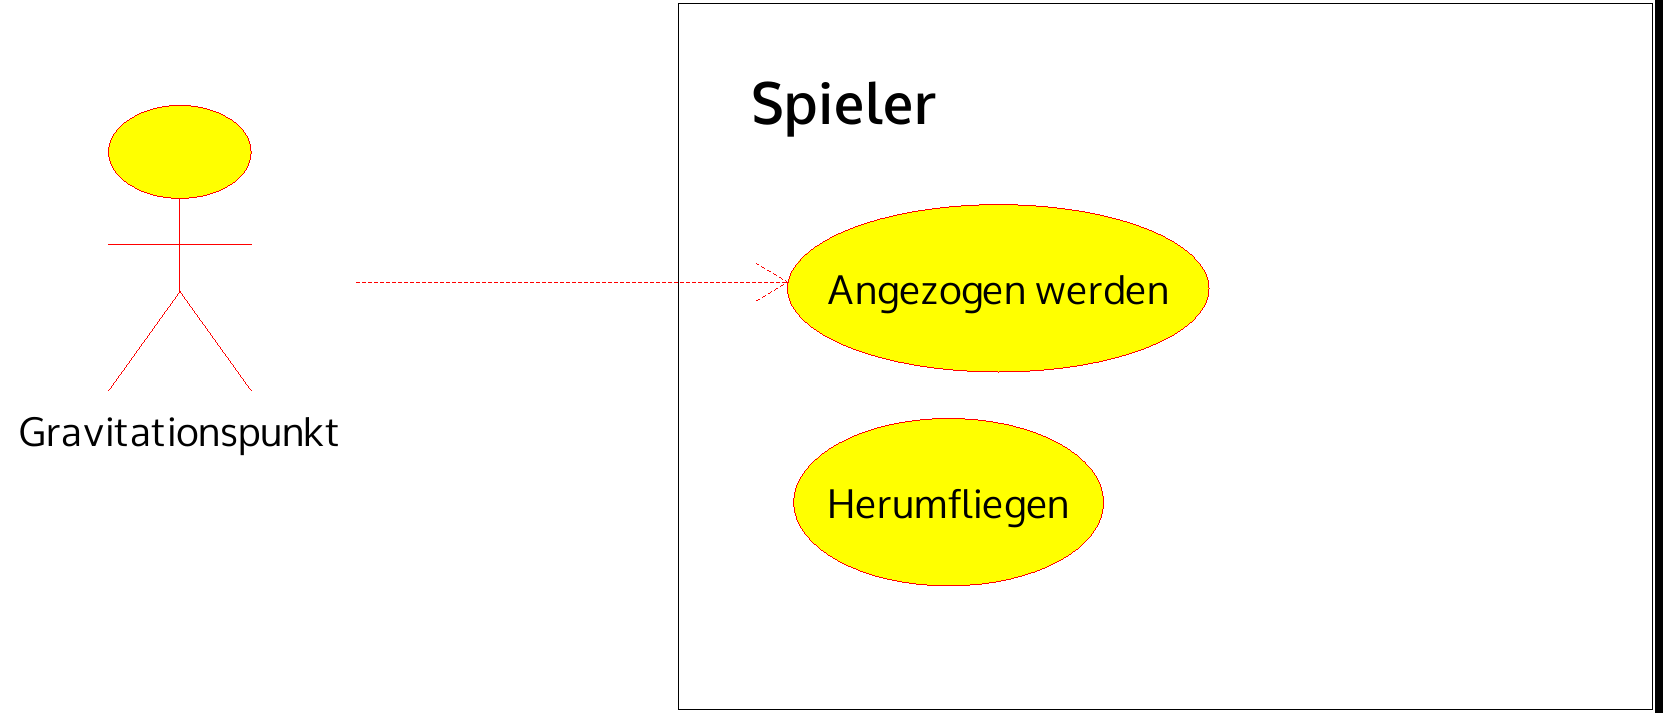
\includegraphics[scale=0.2]{use_cases/spieler.png}


\subsubsection{spaceObject}
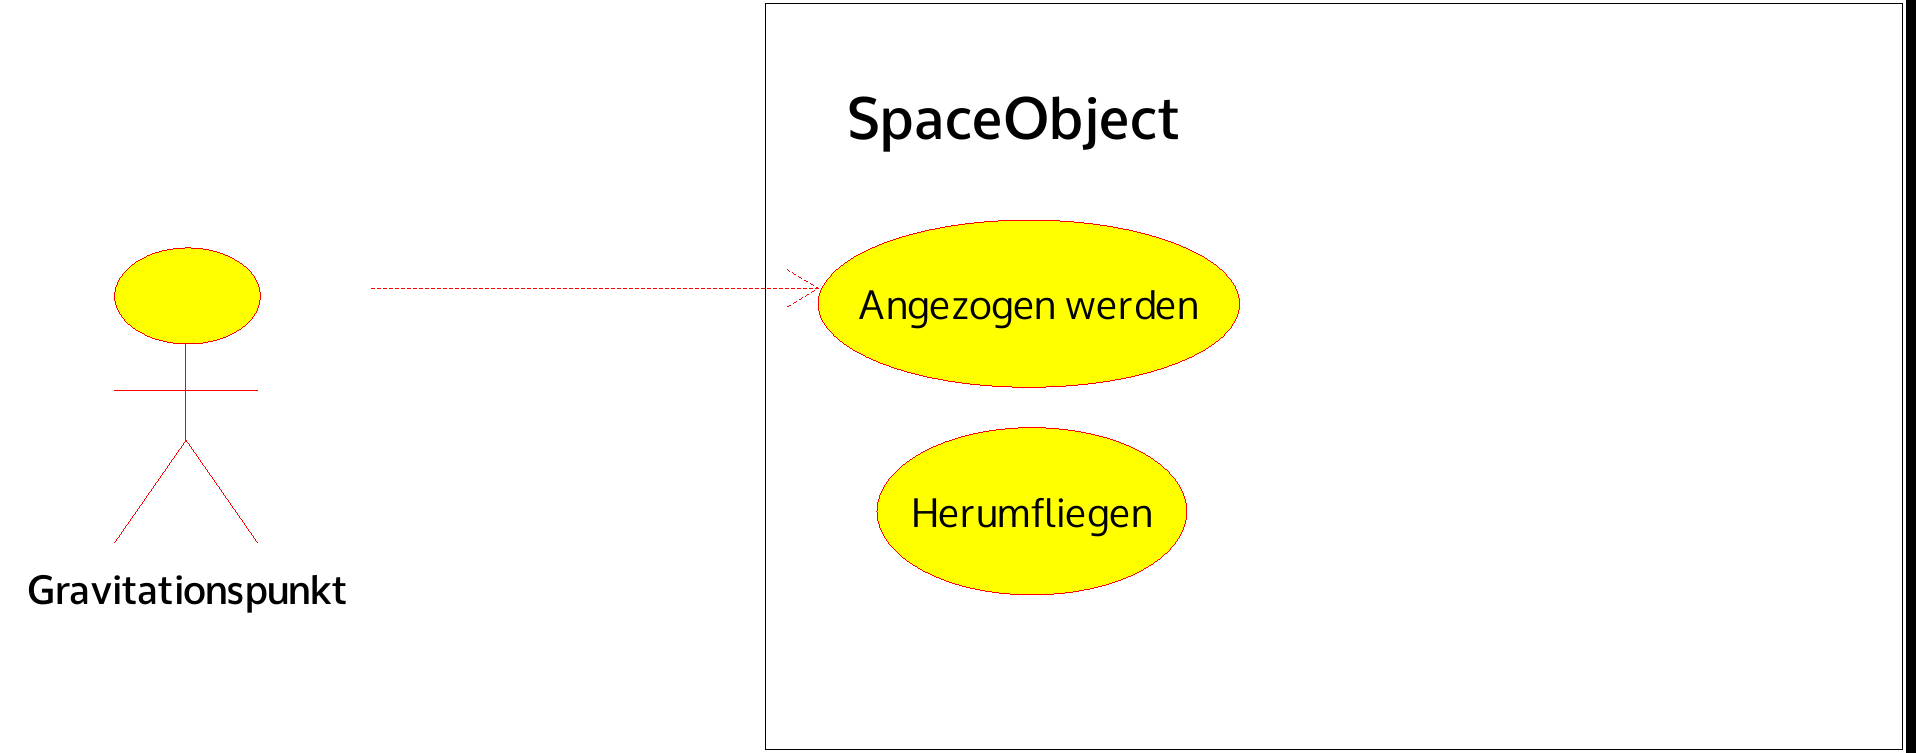
\includegraphics[scale=0.2]{use_cases/spaceObject.png}\\
Ein spaceObject kann von einem Actor (Gravitationspunkt) angezogen werden. Das spaceObject
\q{fliegt} aber jeder Zeit \q{herum}. Dazu braucht es keinen Actor.


\subsection{Anforderungen}
\subsubsection{Technische Ausführung}
\begin{itemize}
\item Mit der Maus soll das Setzen eines Gravitationspunktes - und damit die Steuerung der Spielfigur - möglich sein.
\item Java packages: \begin{itemize}
	\item java.util.* \textit{(Datenstrukturen)}
	\item java.io.* \textit{(Um Daten aus dem .jar als Streams zu laden)}
\end{itemize}
\item JSFML packages: \begin{itemize}
	\item org.jsfml.Graphics.* \textit{(Grafik-API von JSFML)}
	\item ...
\end{itemize}
\end{itemize}
	%% technische ausführung
%4.3 eigene dokumentation - erklären wie das erstellt wurde, darauf verweisen



\section{Entwurf}
\inmilestonetwo
\section{Implementierung}

\section{Resultate und Testen}
\inmilestonetwo
\section{Diskussion und Ausblick}
\inmilestonetwo


% Addendum: Quellcode
%\section{Quellcode}
\subsection{Über unseren Quellcode}
Unser Code ist modular aufgebaut, d.h. das Spiel besteht aus verschiedenen Klassen. Jede Klasse
verfügt über eine eigene Datei.
\subsection{Level.java}
\lstinputlisting[language=Java,breaklines=true,numbers=left,tabsize=4]{../../src/spacetraveler/Level.java}

\end{document}
 
